% ---------------------------------------------------- %
%                CONFIGURATION                         %
% ---------------------------------------------------- %

\documentclass[twoside]{article}

\usepackage{lipsum} % Package to generate dummy text throughout this template
\usepackage{amsmath}
\usepackage[sc]{mathpazo} % Use the Palatino font
\usepackage[T1]{fontenc} % Use 8-bit encoding that has 256 glyphs
\linespread{1.05} % Line spacing - Palatino needs more space between lines
\usepackage{microtype} % Slightly tweak font spacing for aesthetics
\usepackage[hmarginratio=1:1,top=32mm,columnsep=20pt,left=0.8in,right=0.8in]{geometry} % Document margins
\usepackage{multicol} % Used for the two-column layout of the document
\usepackage[hang, small,labelfont=bf,up,textfont=it,up]{caption} % Custom captions under/above floats in tables or figures
\usepackage{booktabs} % Horizontal rules in tables
\usepackage{float} % Required for tables and figures in the multi-column environment - they need to be placed in specific locations with the [H] (e.g. \begin{table}[H])
\usepackage{hyperref} % For hyperlinks in the PDF

\usepackage{lettrine} % The lettrine is the first enlarged letter at the beginning of the text
\usepackage{paralist} % Used for the compactitem environment which makes bullet points with less space between them

\usepackage{abstract} % Allows abstract customization
\renewcommand{\abstractnamefont}{\normalfont\bfseries} % Set the "Abstract" text to bold
\renewcommand{\abstracttextfont}{\normalfont\small\itshape} % Set the abstract itself to small italic text

\usepackage{titlesec} % Allows customization of titles
\renewcommand\thesection{\Roman{section}} % Roman numerals for the sections
\renewcommand\thesubsection{\Roman{subsection}} % Roman numerals for subsections
\titleformat{\section}[block]{\large\scshape\centering}{\thesection.}{1em}{} % Change the look of the section titles
\titleformat{\subsection}[block]{\large}{\thesubsection.}{1em}{} % Change the look of the section titles

\usepackage{fancyhdr} % Headers and footers
\pagestyle{fancy} % All pages have headers and footers
\fancyhead{} % Blank out the default header
\fancyfoot{} % Blank out the default footer
\fancyhead[C]{Efficient Coding Hypothesis and an Introduction to Information Theory $\star$ September 2014} % Custom header text
\fancyfoot[RO,LE]{\thepage} % Custom footer text

\usepackage{graphicx}


% ---------------------------------------------------- %
%                CONFIGURATION                         %
% ---------------------------------------------------- %



% ---------------------------------------------------- %
%                   	TITLE                          %
% ---------------------------------------------------- %

\title{\vspace{-15mm}\fontsize{24pt}{10pt}\selectfont\textbf{Efficient Coding Hypothesis and an introduction to information Theory}} % Article title
\author{Lay Kuan Loh \& Mihovil Bartulovic}
\date{\today}

% ---------------------------------------------------- %
%                   	TITLE                          %
% ---------------------------------------------------- %



\begin{document}

\maketitle % Insert title

\thispagestyle{fancy} % All pages have headers and footers




% ---------------------------------------------------- %
%                   	ABSTRACT                       %
% ---------------------------------------------------- %

\begin{abstract}

\noindent The Efficient Coding Hypothesis, proposed by Barlow 1961, suggests that sensory relays recode sensory messages, so that their redundancy is reduced, but little information is lost. Coding to reduce redundancy not just eliminates wasteful neural activity, but also organizes sensory information such than an internal model of the environment causing the pst sensory inputs ins built up, while the current sensory situation is represented in a way that simplified the task of the parts of the nervours ssystem responsible for learning and conditioning. To investigate animals' sensory mechanisms, Barlow 1961 suggests that one examine the ways in which animals use their senses, as these ways are likely reflected in the design of the sense organs and their nervous pathways.

\end{abstract}

% ---------------------------------------------------- %
%                   	ABSTRACT                       %
% ---------------------------------------------------- %








% ---------------------------------------------------- %
%                   	INTRODUCTION                   %
% ---------------------------------------------------- %

\begin{multicols}{2} % Two-column layout throughout the main article text

\section{Introduction}

\lettrine[nindent=0em,lines=3]{I}nformation Theory represents the necessary basis of the modern information and communication technologies. Without it many of today’s technologies would be unavailable or severely less developed so one can freely say that Information Theory is inextricably woven into the life of a modern man and society.

Information Theory uses bits as a standard choice of units for information.
The core theorems of Information Theory set measure for the quantity of information, upper bound for lossless compression of information as well as the upper speed limit for information transfer trough a channel with or without noise. Even though Information Theory in its core does not give practical solutions for upper bounds that it sets, theoretical basis of it are vital step to practical implementation.  In general, the transfer of information should be fast, precise, energy efficient and it should work regardless the inevitable interference and noises in the channel. Information Theory presents the theoretical foundation so one can achieve such goals and it presents the necessary basis for coding and compressing all types of information (text, images, music, etc.). While coding information it is it is important that it is coded efficiently and this is where the Efficient Coding Hypothesis comes in. 

Efficient Coding Hypothesis is one of the quantitative links between the statistical and structural properties our Visible surroundings. It is highly related to the Information Theory as well as Neuroscience and it has been in the main topic in some of the recent review articles as well as workshops. 
From a Neuroscientific point of view this hypothesis states that a group of neurons should encode information as compactly as possible, so they can use the available resources in the most efficient way. This being said, one can now decouple this statement into two separate statements; one regarding the statistics of a response of single neuron and second regarding the responses of a group of neurons. 

For the case of a single neuron, the output capacity should be fully utilized i.e. the information from one neuron should not be redundant to the information which is carried by the other neurons. 

Testing the Efficient Coding Hypothesis is quite impractical as for the estimation of information-theoretic quantities large amounts of data are required and all of the common estimators of information are heavily biased. Nonetheless, successful experimental results have been achieved.



% ---------------------------------------------------- %
%                   	INTRODUCTION                   %
% ---------------------------------------------------- %



% ---------------------------------------------------- %
%                      BARLOW 1961                     %
% ---------------------------------------------------- %

\section{Possible Principles Underlying the Transformations of Sensory Messages}

H.B. Barlow in his article “Possible Principles Underlying the Transformations of Sensory Messages” discusses three hypotheses about sensory relays:
\begin{itemize}
	\item Sensory relays are for detecting, in the incoming messages, certain ``passwords'' that have a particular key significance.
	\item Sensory relays are filters whose “pass characteristics” can be controlled in accordance with the requirements of the other part of the nervous system.
	\item Sensory relays recode sensory messages, extracting signals of high relative entropy from the highly redundant sensory input.
\end{itemize}

Even though these ideas come from experimental results, not merely from abstract speculation this paper lacks discussion about the experimental evidence behind these ideas i.e. the first hypothesis comes from the realization that frog’s retina had an organization that made it severely unsuitable for the kind of tasks we use our eyes for. 

In the "passwords" hypothesis, it is stated that specific classes of stimuli act as ``releasers'' and evoke specific responses. These classes of stimuli are thought of as “passwords” which have to be distinguished from other stimuli and it is suggested that their detection may be the important function of sensory relays. 

For example, frog’s visual system has a limited range of visual responses. A moving object elicits a sequence of reactions which can be anything between alert for the frog to hopping forward and snapping at it. 

In the Controlled Pass-Characteristic Hypothesis sensitivity of one type of stimulus might be increased while another is decreased, or if this hypothesis is combined with the ``password'' hypothesis the whole characteristic of relay could change, so that, in effect, the ``password'' is altered. 
Write about redundancy reducing hypothesis. 

% ---------------------------------------------------- %
%                      BARLOW 1961                     %
% ---------------------------------------------------- %



% ---------------------------------------------------- %
%                	NIRENBERG 2001                     %
% ---------------------------------------------------- %

\section{Retinal ganglion cells act largely as independent encoders}

\footnotesize
Correlated firing among neurons is widespread in the visual system, but its importance for encoding visual information is unclear. To study this, Nirenberg et. al., 2001 presented the retina with natural stimuli and computed the responses of the output cells, the ganglion cells. They used information theoretic techniques to measure the amount of information about the stimuli that can be obtained from the cells under correlated firing and non-correlated firing. They found that more than 90\% of the information about the stimuli can be obtained from the cells with uncorrelated firing, suggesting that ganglion cells act largely independently to encode information, simplifying the problem of decoding their activity. 

\normalsize
Nirenberg et. al., 2001 stimulated pairs of isolated mouse retina using natural movies. The stimuli were each 7 seconds long and repeated 300 times, and the ganglion cell responses were recorded. Data used had to be clean of contaminating spikes from other cells, and that both responses had to have average firing rates. 

To find the degree of correlated activity for each pair, the excess correlated fraction (ECF) was found. ECF is the fraction of correlated spikes produced by the pair above chance, taking into account correlations induced by the stimulus. The ECFs ranged from -1\% to 34\%. 

To measure the amount of information the pairs of ganglion cells carried about the stimuli when their correlations were taken into account, information theoretic techniques were used. Each movie was treated as a series of segments of fixed temporal length, with each segment regarded as a separate stimulus. The movie was presented several hundred times to generate a large set of responses (spike trains) to each segment. This allowed the authors to estimate the probability of getting a particular pair of responses given a particular movie segment - that is, to estimate $\mathbb{P}(r_1,r_2|s)$, where $r_1$ was the response of cell 1, $r_2$ was the response of cell 2 and $s$ was the movie segment. Given these conditional probabilities, the amount of information $I$ between the responses and the stimulus segments was found using the expression:


\begin{align}\label{eq:info-theory}
	I 
		&= -\sum_{r_1,r_2}\mathbb{P}(r_1,r_2)\log_2\mathbb{P}(r_1,r_2) \\
  		&+ \sum_s\mathbb{P}(s) \sum_{r_1,r_2}\mathbb{P}(r_1,r_2|s)\log_2\mathbb{P}(r_1,r_2|s)
\end{align}


where $\mathbb{P}(r_1,r_2)$ is found by taking $\mathbb{P}(r_1,r_2) = \sum_s \mathbb{P}(r_1,r_2|s)\mathbb{P}(s)$, and $\mathbb{P}(s)$ is the probability that a given stimulus segment $s$ occured. 

To examine how important correlation is in encoding visual information, the amount of information that would be lost if the correlations in the responses of the pair of ganglion cells were ignored was examined. To ignore the correlations, the conditional probability distributions of the two responses, $\mathbb{P}(r_1,r_2|s)$, as the product of their individual probability distributions, $\mathbb{P}(r_1|s)$ and $\mathbb{P}(r_2|s)$. $\mathbb{P}(r_1|s)\mathbb{P}(r_1|s)$ to estimate the probability of a stimulus given a response. As $\mathbb{P}(r_1|s)\mathbb{P}(r_1|s)$ is not quite the true distribution, using it should lead to a loss of information. 

Therefore, the amount of independent information is given by

\begin{align}
	I_{IND} 
		&= -\sum_{r_1,r_2}\mathbb{P}(r_1,r_2|s)\log_2\mathbb{P}(r_1|s)\mathbb{P}(r_2|s) \\
		&+ \sum_s\mathbb{P}(s) \sum_{r_1,r_2}\mathbb{P}(r_1,r_2|s)\log_2\mathbb{P}(r_1|s)\mathbb{P}(r_2|s) 
\end{align}

The amount of information in bits lost, $\Delta I$, is given by 
\begin{align}
	\Delta I 
		&= I - I_{IND} \\
		&= \sum_s\mathbb{P}(s) \sum_{r_1,r_2}\mathbb{P}(r_1,r_2|s) \log_2 \frac{\mathbb{P}(r_1,r_2|s)}{\mathbb{P}(r_1|s)\mathbb{P}(r_2|s)} \\
		&- \sum_{r_1,r_2}\mathbb{P}(r_1,r_2) \log_2 \frac{\mathbb{P}(r_1,r_2)}{\sum_s \mathbb{P}(r_1|s)\mathbb{P}(r_2|s) \mathbb{P}(s)} 
\end{align}

$\Delta I$ is very small, as most pairs lost less than 10\% of information. If there were pairs of ganglion cells with higher degrees of correlation than the maximum 34\% observed, more information loss could have occured. This finding means that strategies used to decode ganglion cell activity, which treat the cells as independent encoders are reasonable, as they can capture more than 90\% of the information the cells carry. Furthermore, the activity of any given ganglion cell can be evaluated separately from other cells, without accounting for other cells in the population. This allows the problem of decoding population activity to be significanly simplified, as much less data is needed to analyze the uncorrelated case as opposed to the correlated case. 

Several concerns with the study are that capturing more than 90\% in ganglion cell activity may not be enough to fully understand its activity. Also, perhaps correlation should not be ignored for the activity of a larger population of cells than just pairs of cells studied here. 

% ---------------------------------------------------- %
%                	NIRENBERG 2001                     %
% ---------------------------------------------------- %





% ---------------------------------------------------- %
%                    LAUGHLIN 1981                     %
% ---------------------------------------------------- %

\section{A Simple Coding Procedure Enhances a Neuron's Information Capacity}

This study by Laughlin 1981 validates Barlow 1961's suggestion that redundancy reduction is an important principle in neural coding. Laughlin that the receptors of large monopolar cells (LMCs), the first order interneurons of the insect compound eye, have a compressive intensity-response function corresponding to the background intensity. Instead of absolute intensity, the LMC's contrast-response function matches the range of contrasts encountered in natural scenes, which increases the efficiency.

A neuron has a limited range of responses that can represent the states of its inputs. If its sensitivities are too high, inputs would saturate the response, and input outside the response range would be lost. If sensitivities are too low, the response range would correspond to very large ranges of input, and many parts of it would therefore be underutilized. Information theory suggests that the most efficient way to apportion the neuron's limited response range is to maximize entropy by encoding inputs so that all response levels are used with equal frequency. 

In the simplest case, shown in Figure~\ref{fig:laughlin1981-fig1}, a neuron represents a single input parameter with a single output parameter. Maximum entropy is achieved when inputs are amplified in proportion to their expected frequeny of occurence. Larger portions of the response range are used for better resolution of common events, and smaller portions for improbable events. 

\begin{figure}[H]
	\caption{
		\textsc{Upper diagram:} Probability density function for stimulus intensities. \\ \textsc{Lower diagram:} Intensity-response function that implements the strategy. \\ Maxmimizing a neuron's information capacity by ensuring that all response levels are used with equal frequency. Intervals between each response level encompasses an equal area under the intensity distribution, so each state is used with equal frequency.
	}
	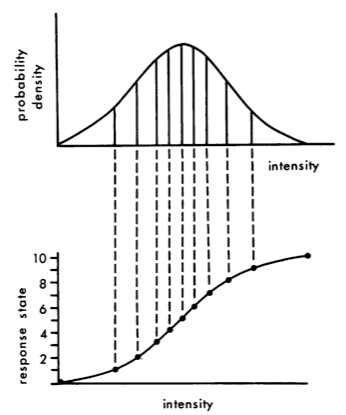
\includegraphics[width=0.45\textwidth]{laughlin1981-fig1}
	\label{fig:laughlin1981-fig1}
\end{figure}

To test this hypothesis, Laughlin compared contrast-response functions with contrast levels measured in natural scenes, such as lakeside vegetation in LMCs. Relative intensities were measured accross the scenes with a detector with spectral sensitivity similar to a fly monopolar cell. Contrast values were obtained by dividing each scan into intervals. Within each interval, the intensity $\bar{I}$ was found, and for each data point the fluctuation about the mean $\delta I = I - \bar{I}$ was computed. Finally, the contrast $\displaystyle\frac{\Delta I}{\bar{I}}$ was found. The contrast-response function approximates the form of the cumulative distribution function for contrast levels in natural scenes~\ref{fig:laughlin1981-fig2}, indicating that the neurons uses the strategy for efficient coding suggested by information theory. Therefore, there is little redundancy associated with the LMC response to natural scenes. 

\begin{figure}[H]
	\caption{
		The contrast-response function of light adapted fly LMCs compared to the cumulative probability function for natural contrasts ($50^\circ$ interval).
	}
	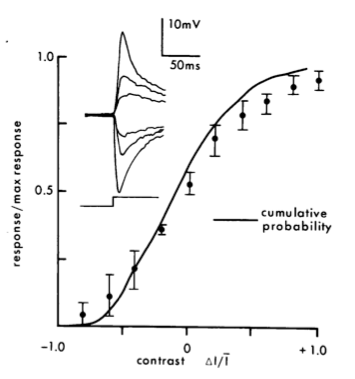
\includegraphics[width=0.45\textwidth]{laughlin1981-fig2}
	\label{fig:laughlin1981-fig2}
\end{figure}

% ---------------------------------------------------- %
%                    LAUGHLIN 1981                     %
% ---------------------------------------------------- %



% ---------------------------------------------------- %
%                     SIMONCELLI 2003                  %
% ---------------------------------------------------- %

\section{Vision and the Statistics of the Visual Environment}

Eero P. Simoncelli in his paper titled ``Vision and the statistics of the visual environment'' brings several criticisms about Efficient Coding Hypothesis. His review puts stress on the efficient coding articles published in the last several years. The author argues some misconceptions about the theory or variants of theory behind Efficient Coding Hypothesis. Several criticisms are regarding experimental and fundamental issues of the Efficient Coding Hypothesis.

\subsection{Criticisms}

First issue which this review rises is that the efficient coding of visual information is not important. The base of this criticism lies in questioning the purpose of vision. The author argues that the purpose of vision is not to encode and reconstruct the visual world. However, it is not mentioned how the extracted information is being used afterwards. 
Second criticism of the Efficient Coding Hypothesis is that the Information Theory from Neuroscientific standpoint is not important because brain does not work with bits. 

Next criticism of the Efficient Coding Hypothesis touches the experimental data of multi neuron recordings. Some data show correlation as well as synchronization or some other form of statistical dependency between neurons.  However, the author disproves this criticism by saying that the experimental data did not use naturalistic stimuli and thus the data is not directly relevant to the hypothesis. Even in the case of a naturalistic stimulus the hypothesis states that the system tends to be independent. 

Furthermore, the Efficient Coding Hypothesis is criticized based on the comparison between the numbers of retinal ganglion cells to the number of neurons in the primary visual cortex. It is argued that the number of neurons which are used to process sensory information is expanding as the information goes deeper into the system thus brain increases redundancy by itself.  It is assumed that the coding capacity of all neurons is the same. Still, increased number of neurons does not always yield redundancy as different neurons have different properties i.e. cortical neurons have slower firing rate and they tend to have more complex temporal dynamic properties. The redundancy for retinal and V1 neurons has not yet been experimentally compared a similar comparison in auditory system demonstrated the reduction of redundancy. 
The theory behind Efficient Coding Hypothesis uses several assumptions – it strongly dependent on probability distribution of natural images and the definition of the neural response.  This is the most fundamental problem for the Efficient Coding Hypothesis. In a usual scenario the distribution of inputs is not defined but it is assumed to be represented with a collection of calibrated images. Also, while applying the hypothesis one must explicitly denote which neurons are used to satisfy it. 

The last criticism of Efficient Coding Hypothesis discussed in this paper is that the commonly used versions of the theory ignore noise and other simplistic physical constraints. Even though this criticism is a valid one it is not looked upon as a fatal one. 

\subsection{Testing the hypothesis}

Efficient Coding Hypothesis, even though being about 50 years old, is only being more explored. Today, we have greater knowledge of early sensory processing, better mathematical and engineering tools so we can manipulate with more complex statistical models and we can gather and process large amounts of data used in experimental stimuli and statistical purposes. 
There are two basic approaches for testing the Efficient Coding Hypothesis. Frist one focuses on examining statistical properties of neural responses under natural stimuli. On the other hand the second one focuses on using statistical properties of natural images to constrain and derive a model for the early sensory processing.

In the last few years researchers have been able to measure the efficiency in several different ways. Results of those studies vary – some studies confirm the Efficient Coding Hypothesis and the others seem to be highly inconsistent with the proposed hypothesis.  In example, a study conducted on cats and monkeys has shown that firing rate distributions of cat’s visual V1 and monkey’s inferotemporal (IT) neurons is exponential under naturalistic conditions and this yields optimal information transmission for a fixed average rate of firing. Furthermore, another study with monkey’s IT neurons found that only minority could be described with an exponential firing distribution. Later, it was argued that exponential distribution is a correct solution only in noise-free cases (cite 28,39,40). 

In a study presented in (cite 41) it was shown that retinal ganglion cells show strong firing correlations and that the observed patterns could provide useful information.  Article by (cite 23) adds that retinal ganglions cells act as an independent encoders. Similar result for V1 neurons was found by (cite 42) where it was stated that V1 neurons are almost independent under non-natural stimuli. Results mentioned so far can seem not in line with the Efficient Coding Hypothesis as one would expect the level of independency to degrade for non-natural stimuli. 

(cite 44 and 45 ) suggest that visual system shows better performance while input is a naturalistic stimulant. 

Even though the connection has not yet been completely established, Efficient Coding Hypothesis suggests that optimal characterization of neural system will be while using natural stimuli.

On the other hand, the other method of testing the Efficient Coding Hypothesis is to derive a model for efficient coding of the environment and afterwards to compare it with the observed psychological data. This model is highly constrained with linear filtering and second order statistical modeling. In the last few years, a couple of authors have established a connection between higher order statistical model and linear filtering.

Finally, it is worth mentioning that several authors successfully applied Efficient Coding Hypothesis to adaptive processes.

The recent interest in Efficient Coding Hypothesis has given interesting theoretical and experimental results. After all this being said it does seem improbable that Efficient Coding Hypothesis will be sufficient and the only principle for the understanding of sensory system design but it is clear that this hypothesis will play an important role.


% ---------------------------------------------------- %
%                     SIMONCELLI 2003                  %
% ---------------------------------------------------- %







% ---------------------------------------------------- %
%                 	REFERENCE LIST                     %
% ---------------------------------------------------- %

\begin{thebibliography}{99} 

\bibitem[Barlow 1961]{Barlow:1961dg}
Barlow, H.~B. (1961).
\newblock Possible Principles Underlying the Transformations of Sensory Messages.
\newblock {\em Sensory communication}, (1961):217-234.

\bibitem[Laughlin, 1981]{Laughlin:1981dg}
Laughlin, S. (1981).
\newblock A Simple Coding Procedure Enhances a Neuron's Information Capacity.
\newblock {\em Z. Naturforsch}, 36.910-912 (1981): 51.

\bibitem[Nirenberg et. al., 2001]{Nirenberg:2001dg}
Nirenberg, S., Carcieri, S.~M., Jacobs, A.~L., \& Latham, P.~E. (2001).
\newblock Retinal ganglion cells act largely as independent encoders.
\newblock {\em Nature}, 411(6838), 698-701.

\bibitem[Simoncelli 2003]{Simoncelli:2003dg}
Simoncelli, E.~P. (2003).
\newblock  Vision and the statistics of the visual environment.
\newblock {\em Current opinion in neurobiology}, 13(2), 144-149.
 
\end{thebibliography}

% ---------------------------------------------------- %
%                 	REFERENCE LIST                     %
% ---------------------------------------------------- %


\end{multicols}

\end{document}


% ---------------------------------------------------- %
